% !TEX program = xelatex
\documentclass[UTF8,a4paper,zihao=-4,fontset=none]{ctexart}

\usepackage[a4paper,top=2.4cm,bottom=2.2cm,left=2.4cm,right=2.4cm]{geometry}
\usepackage{fontspec}
\usepackage{xeCJK}
\usepackage{amsmath,amssymb}
\usepackage{graphicx}
\usepackage{booktabs}
\usepackage{array}
\usepackage{multirow}
\usepackage{enumitem}
\usepackage{caption}
\usepackage{float}
\usepackage{hyperref}

\IfFontExistsTF{Times New Roman}{\setmainfont{Times New Roman}}{\setmainfont{TeX Gyre Termes}}
\IfFontExistsTF{SimSun}{
  \setCJKmainfont[
    BoldFont=SimHei,
    ItalicFont=KaiTi
  ]{SimSun}
}{
  \setCJKmainfont{FandolSong}
}
\setmonofont{Courier New}

\hypersetup{
  colorlinks=false,
  pdfborder={0 0 0},
  pdftitle={EDM-StructLoRA: 面向电子音乐生成的结构与属性感知参数高效适配方法},
  pdfauthor={作者姓名}
}

\ctexset{
  section = {
    format = \zihao{4}\bfseries,
    name = {,、},
    number = \chinese{section},
    aftername = \hspace{0pt}
  },
  subsection = {
    format = \zihao{-4}\bfseries,
    name = {,、},
    number = \arabic{section}.\arabic{subsection},
    aftername = \hspace{0.5em}
  },
  subsubsection = {
    format = \zihao{-4}\bfseries,
    name = {,、},
    number = \arabic{section}.\arabic{subsection}.\arabic{subsubsection},
    aftername = \hspace{0.5em}
  }
}

\captionsetup{font=small,labelfont=bf}
\setlength{\parindent}{2em}
\setlength{\parskip}{0pt}
\linespread{1.18}
\sloppy

\newcommand{\modelname}{EDM-StructLoRA}
\newcommand{\basemodel}{ACE-Step}
\newcommand{\datasetname}{EDM-Adapter}

\title{\bfseries \modelname：面向电子音乐生成的结构与属性感知参数高效适配方法}
\author{作者姓名\\单位名称\\邮箱}
\date{}

\begin{document}
\maketitle

\begin{abstract}
文本生成音乐模型已经能够根据自然语言提示生成完整音频片段，但在电子舞曲（Electronic Dance Music, EDM）场景中仍面临结构控制不足的问题。EDM 的创作依赖明确的段落组织、稳定的 BPM、可感知的能量变化、低频冲击和循环边界，而通用文本提示往往难以稳定约束这些时间相关属性。针对这一问题，本文提出 \modelname，一种面向 EDM 生成的结构与属性感知参数高效适配框架。该方法基于 \basemodel 音乐生成基础模型，将传统单一 LoRA 扩展为共享 EDM LoRA、段落专家 LoRA、能量专家 LoRA 和子风格专家 LoRA，并通过元数据路由器在训练与推理阶段动态计算 adapter mixture。进一步地，本文构建 latent-frame aligned control curve，将 section、subgenre、energy、BPM、beat phase、low-frequency ratio、onset density、loop boundary 和标签置信度编码为 36 维帧级控制信号，再通过轻量 MLP control conditioner 转换为额外文本条件 token 注入扩散 Transformer。实验原型构建了 231 个原始音频源、203 个有效处理源和 6,016 条 8 秒 EDM 训练片段，生成对应的 ACE-Step latents、text tokens 和控制曲线，并完成 HuggingFace Dataset 转换、LoRA bundle 保存和可控推理流程。与普通 LoRA 微调相比，本文方法的核心优势在于将 EDM 领域结构知识显式纳入参数高效适配过程，为 BPM、段落、能量与子风格可控的文本生成音乐提供了一条可复现的工程路径。
\end{abstract}

\noindent\textbf{关键词：}文本生成音乐；电子舞曲；LoRA；可控生成；Adapter Routing；Control Token；ACE-Step

\vspace{0.6em}
\noindent\textbf{Abstract:}
Text-to-music models can synthesize musical audio from natural-language prompts, but they still lack reliable structural control for electronic dance music (EDM). EDM production depends on explicit sections, stable BPM, energy progression, bass impact, onset density and loop boundaries, which are difficult to constrain by text prompts alone. This paper presents \modelname, a structure- and attribute-aware parameter-efficient adaptation framework for controllable EDM generation. Built on the \basemodel foundation model, \modelname replaces a single fixed LoRA adapter with a shared EDM adapter, section experts, energy experts and subgenre experts. A metadata-conditioned router dynamically activates adapter mixtures during training and inference. In addition, a latent-frame aligned control curve encodes section, subgenre, energy, BPM, beat phase, low-frequency ratio, onset density, loop markers and confidence values into 36-dimensional frame-level controls, which are projected into additional text-conditioning tokens. The prototype builds 6,016 cleaned 8-second EDM clips from 231 raw sources, caches ACE-Step latents, constructs control assets and implements a full training-inference pipeline. The proposed framework explicitly injects EDM structural knowledge into parameter-efficient adaptation and provides a reproducible path toward controllable text-to-EDM generation.

\noindent\textbf{Keywords:} text-to-music generation; EDM; LoRA; controllable generation; adapter routing; control token; ACE-Step

\section{引言}

近年来，文本生成音频与文本生成音乐模型快速发展。MusicLM、MusicGen、AudioLDM 以及 ACE-Step 等模型表明，基于大规模音频数据和强表征模型的生成系统已经能够根据自然语言描述合成具有较高可听性的音乐片段。然而，音乐生成任务并不只是“根据风格词生成声音”。对于电子舞曲，尤其是 festival EDM、melodic house、progressive house、future bass 等类型，生成质量很大程度上取决于段落功能、节奏速度、能量轨迹、低频分布和循环可用性。实际音乐制作中，用户常常需要生成“128 BPM 的 high energy drop”“适合作为 loop 的 tropical house intro”“带有 warm sidechain bass 的 melodic house build-up”。这些需求同时包含文本语义、音乐结构和连续时间属性。

现有通用文本生成音乐模型通常将用户意图压缩进 prompt。该方式在描述风格、乐器和情绪时较为有效，但对 EDM 的结构化属性控制仍不稳定。首先，模型可能无法稳定区分 intro、build-up、drop、breakdown 和 loop 等段落。其次，BPM、鼓点密度、低频能量和 loop 边界是时间相关信号，单纯写入 caption 并不能保证在生成过程中被精确执行。第三，普通 LoRA 微调一般只训练一个固定 adapter，它可以学习某个领域的整体音色偏移，却难以对不同段落、能量等级和子风格进行差异化建模。

为解决上述问题，本文提出 \modelname。其核心思想是：将 EDM 生成中的“领域适配”从单一风格迁移扩展为结构与属性条件下的动态参数适配。具体而言，模型使用一个共享 LoRA 捕获 EDM 的整体域偏移，同时使用多个低秩专家 LoRA 表征不同 section、energy 和 subgenre。router 根据样本元数据计算 adapter 权重，使模型在处理 drop、intro、loop 等不同输入时激活不同参数子空间。同时，本文设计 36 维 latent 对齐控制曲线，将 BPM、beat phase、onset density、low-frequency ratio 和 loop markers 等时间信息显式注入文本条件序列，使扩散 Transformer 能够同时接收语义条件与结构控制信号。

本文的主要贡献如下：

\begin{enumerate}[leftmargin=2em,itemsep=0.2em]
  \item 提出面向 EDM 生成的结构与属性感知 LoRA 路由框架，将固定 LoRA 扩展为共享 adapter 与多专家 adapter 的动态组合。
  \item 设计 latent-frame aligned EDM control curve，将 section、subgenre、energy、BPM、节拍相位、低频比例、onset 密度、loop 边界与置信度编码为统一控制张量。
  \item 实现控制曲线到文本条件 token 的轻量投影模块，使结构控制以额外 conditioning tokens 的形式注入 ACE-Step 扩散 Transformer。
  \item 构建包含 6,016 条 8 秒训练片段的 EDM 数据处理与训练流水线，覆盖音频切片、标签构建、caption 生成、latent 缓存、HuggingFace Dataset 转换、adapter bundle 保存与可控推理。
\end{enumerate}

\section{相关工作}

\subsection{文本生成音乐}

文本生成音乐模型的研究目标是根据自然语言描述生成符合语义和音乐风格的音频。MusicLM 将文本到音乐生成表述为层次化序列到序列任务，能够生成较长时间尺度的音乐音频。MusicGen 使用压缩离散音频 token 并通过单个语言模型建模多流表示，在文本控制和旋律条件方面表现出较强能力。AudioLDM 将潜空间扩散模型引入文本到音频生成，说明 latent diffusion 对音频合成具有良好扩展性。ACE-Step 进一步面向音乐生成基础模型构建开放式训练与推理框架，适合作为下游风格适配与可控生成研究的基础。

尽管这些模型提升了生成音质和文本相关性，但它们通常不直接面向 EDM 的段落结构进行建模。文本提示可以描述“drop”或“128 BPM”，却很难保证生成片段在低频冲击、鼓点密度、loop 首尾衔接和段落功能上稳定满足要求。因此，本文将研究重点放在通用基础模型之上的 EDM 领域适配和结构控制。

\subsection{可控音乐生成}

可控音乐生成关注如何将节奏、和弦、旋律、音色、参考音频或时间变化属性作为条件注入生成模型。MusiConGen 等工作表明，单纯文本条件不足以精确控制 rhythm 和 chord 等音乐属性，引入自动提取或用户指定的时间条件能够提高生成一致性。ControlNet 在图像扩散模型中展示了保留基础模型能力并引入额外控制分支的思路，该思想对音频生成中的结构控制具有启发意义。

与已有工作不同，本文并未训练一个重型控制网络，而是使用轻量控制 token 投影器和 LoRA adapter routing。该设计更加适合资源受限的研究原型，并且能够利用已有 ACE-Step 权重与缓存 latent 降低训练成本。

\subsection{参数高效微调与 LoRA}

LoRA 通过冻结预训练模型参数并在权重矩阵中加入低秩增量，显著降低大模型微调的训练参数量。给定预训练权重 $W_0 \in \mathbb{R}^{d \times k}$，LoRA 将下游适配表示为：
\begin{equation}
  W = W_0 + \Delta W,\quad \Delta W = \frac{\alpha}{r}BA,
\end{equation}
其中 $A \in \mathbb{R}^{r \times k}$，$B \in \mathbb{R}^{d \times r}$，$r \ll \min(d,k)$。普通 LoRA 通常对应一个固定的 $\Delta W$，适合学习整体域偏移，但在结构化音乐生成中难以表达“同一基础模型在不同段落和属性下应使用不同适配方向”的需求。本文将 LoRA 进一步组织成共享 adapter 和专家 adapter 的集合，并通过 router 动态计算组合权重。

\section{问题定义与需求分析}

给定文本提示 $p$、EDM 控制元数据 $m$ 和基础音乐生成模型 $G_{\theta}$，本文目标是生成音频片段 $x$，使其同时满足文本语义、EDM 子风格、段落功能、目标 BPM、能量等级和 loop 结构约束。元数据可表示为：
\begin{equation}
  m = \{s, e, g, b, q, c\},
\end{equation}
其中 $s$ 表示 section，$e$ 表示 energy，$g$ 表示 subgenre，$b$ 表示 BPM，$q$ 表示样本质量权重，$c$ 表示标签置信度。

从应用角度看，该问题具有以下痛点：

\begin{enumerate}[leftmargin=2em,itemsep=0.2em]
  \item \textbf{段落功能不稳定：}EDM 的 drop、build-up、intro 和 loop 对鼓组、低频与编排密度有不同要求，普通 prompt 难以保证模型稳定区分。
  \item \textbf{BPM 和节奏控制弱：}BPM 属于连续数值属性，beat phase 与 onset density 属于时间相关特征，仅通过自然语言描述会产生执行偏差。
  \item \textbf{能量标签表达粗糙：}high energy 不只是一段文字标签，它应对应更高鼓点密度、更强低频和更明显动态推进。
  \item \textbf{单一 LoRA 适配能力有限：}固定 adapter 容易学习平均风格，难以在不同 section 与 subgenre 间切换适配方向。
  \item \textbf{数据工程复杂：}可控生成需要对音频切片、元数据、caption、latent、control curve 和训练样本格式进行一致管理。
\end{enumerate}

\section{方法}

\subsection{总体框架}

\modelname 的总体框架如图 \ref{fig:architecture} 所示。系统输入由文本提示和 EDM 控制元数据组成。router 根据 section、energy、subgenre、BPM 和置信度计算 LoRA 专家权重，动态激活共享 LoRA 与专家 LoRA。与此同时，控制曲线构建器生成与 latent frame 对齐的 36 维控制序列，control conditioner 将该序列压缩为固定数量的控制 token，并拼接到文本编码器输出之后。最终，ACE-Step 扩散 Transformer 在文本 token、控制 token 和动态 LoRA 参数共同作用下完成音乐片段生成。

\begin{figure}[H]
  \centering
  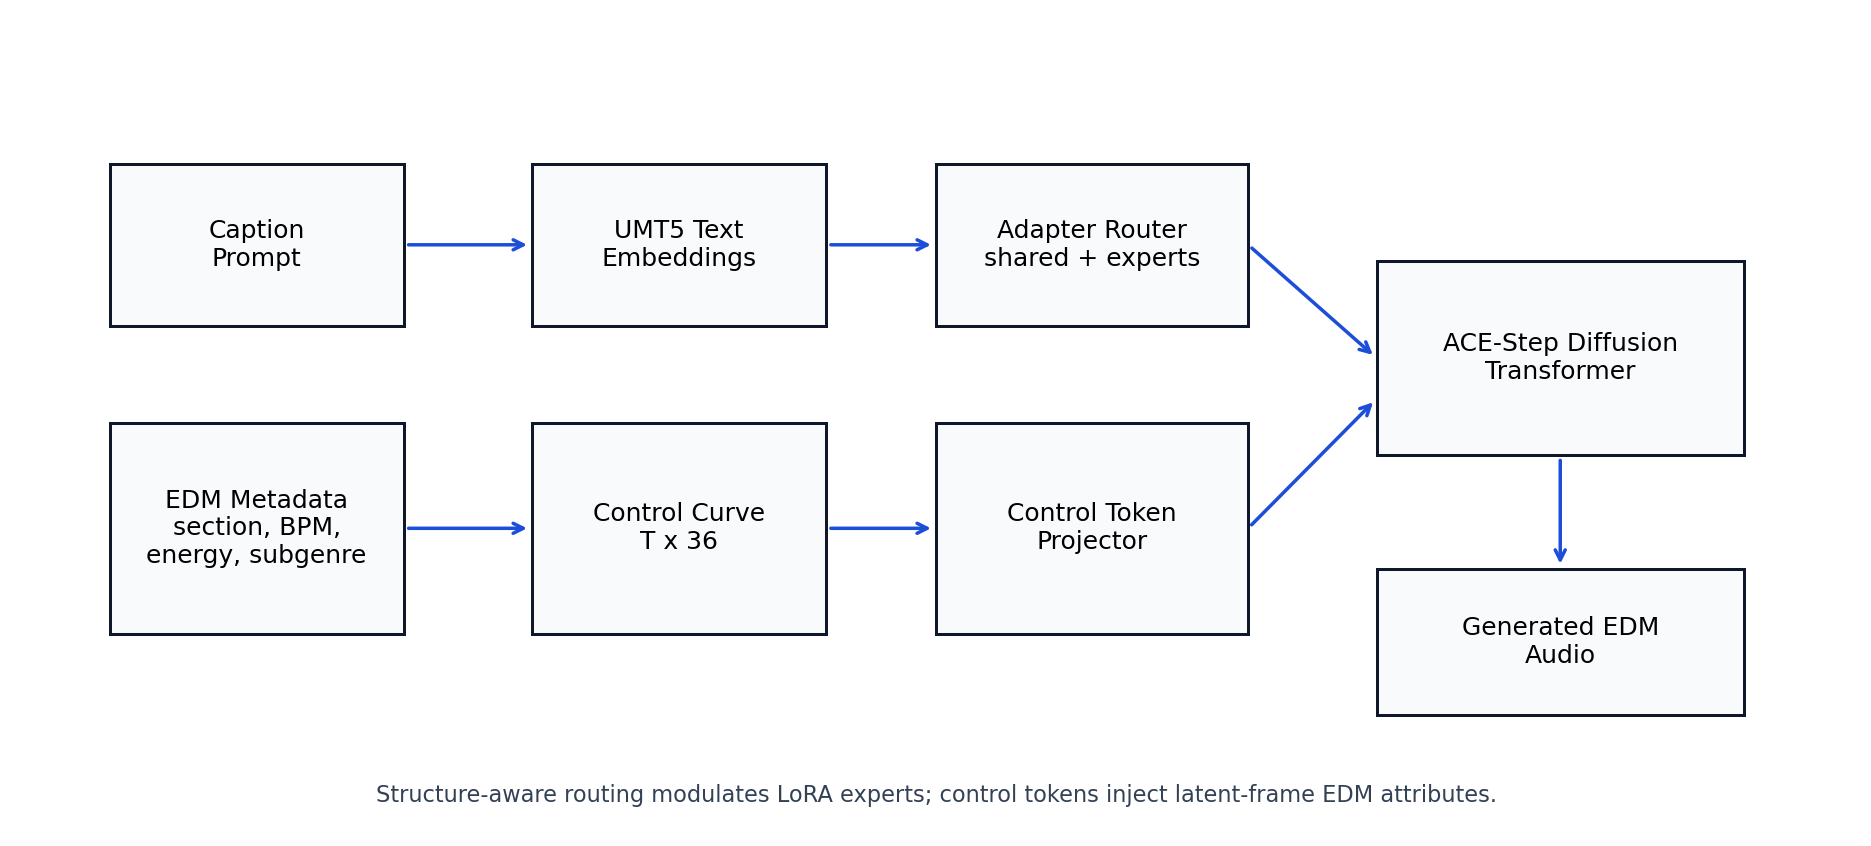
\includegraphics[width=0.92\linewidth]{../paper_assets/fig1_architecture.png}
  \caption{\modelname 总体结构示意图}
  \label{fig:architecture}
\end{figure}

\subsection{结构与属性感知 LoRA 路由}

本文将 LoRA adapter 集合定义为：
\begin{equation}
  \mathcal{A} = \{a_0\} \cup \mathcal{A}_{sec} \cup \mathcal{A}_{ene} \cup \mathcal{A}_{sub},
\end{equation}
其中 $a_0$ 为共享 EDM adapter，$\mathcal{A}_{sec}$ 为 section 专家集合，$\mathcal{A}_{ene}$ 为 energy 专家集合，$\mathcal{A}_{sub}$ 为 subgenre 专家集合。当前实现中包含 1 个共享 adapter、9 个 section experts、4 个 energy experts 和 11 个 subgenre experts，共 25 个 adapter。

对于 batch 中的样本 $i$，router 根据元数据计算权重：
\begin{equation}
  \omega_{a}^{(i)} = f_a(s_i,e_i,g_i,b_i,c_i,q_i),
\end{equation}
batch 级 adapter 权重为：
\begin{equation}
  \bar{\omega}_a = \frac{1}{N}\sum_{i=1}^{N}\omega_{a}^{(i)}.
\end{equation}

在工程实现中，共享 adapter 权重固定为 1.0，section、energy 和 subgenre 专家的权重分别由标签置信度、样本权重和 BPM 偏移进行缩放：
\begin{equation}
  \omega_{sec} = \lambda_s c_s q \left(1 + \lambda_b \frac{|b-128|}{60}\right),
\end{equation}
\begin{equation}
  \omega_{ene} = \lambda_e c_e q \left(1 + \lambda_b \frac{|b-128|}{60}\right),
\end{equation}
\begin{equation}
  \omega_{sub} = \lambda_g c_g q,
\end{equation}
其中 $\lambda_s$、$\lambda_e$、$\lambda_g$、$\lambda_b$ 分别为 section、energy、subgenre 和 BPM scale。当前配置取 $\lambda_s=0.90$、$\lambda_e=0.35$、$\lambda_g=0.45$、$\lambda_b=0.20$。

该路由机制的作用不是替代文本 prompt，而是在参数空间中提供与 EDM 结构相关的适配方向。例如，当输入指定为 high energy melodic house drop 时，系统会同时激活 shared EDM adapter、section\_drop、energy\_high 和 subgenre\_melodic\_house，使模型对 drop 冲击、能量密度和 melodic house 音色进行联合建模。

\subsection{Latent 对齐控制曲线}

为了避免模型只依赖 caption 理解结构属性，本文构建 latent-frame aligned control curve。对于每个音频片段，系统生成控制矩阵：
\begin{equation}
  C = [c_1,c_2,\ldots,c_T] \in \mathbb{R}^{T \times F},
\end{equation}
其中 $T$ 为 latent frame 数，$F=36$ 为控制特征维度。控制特征包括 section one-hot、subgenre one-hot、energy one-hot、energy scalar、normalized BPM、BPM confidence、beat phase sin/cos、time position、low-frequency ratio、onset density、loop start/end markers、tag confidence mean 和 quality weight。

第 $t$ 帧的 beat phase 使用正弦余弦编码：
\begin{equation}
  \phi_t = 2\pi \frac{b}{60}\tau_t,\quad
  c_t^{phase} = [\sin(\phi_t), \cos(\phi_t)],
\end{equation}
其中 $b$ 为 BPM，$\tau_t$ 为第 $t$ 个 latent frame 对应的音频时间。该编码使模型能够获得连续节拍位置信息，而不是仅接收离散 BPM 标签。

图 \ref{fig:control_curve} 展示了控制曲线在不同特征维度上的变化。与传统 caption-only 微调相比，控制曲线能够显式表达时间位置、节拍相位和 loop 边界，从而增强生成过程对节奏结构的感知。

\begin{figure}[H]
  \centering
  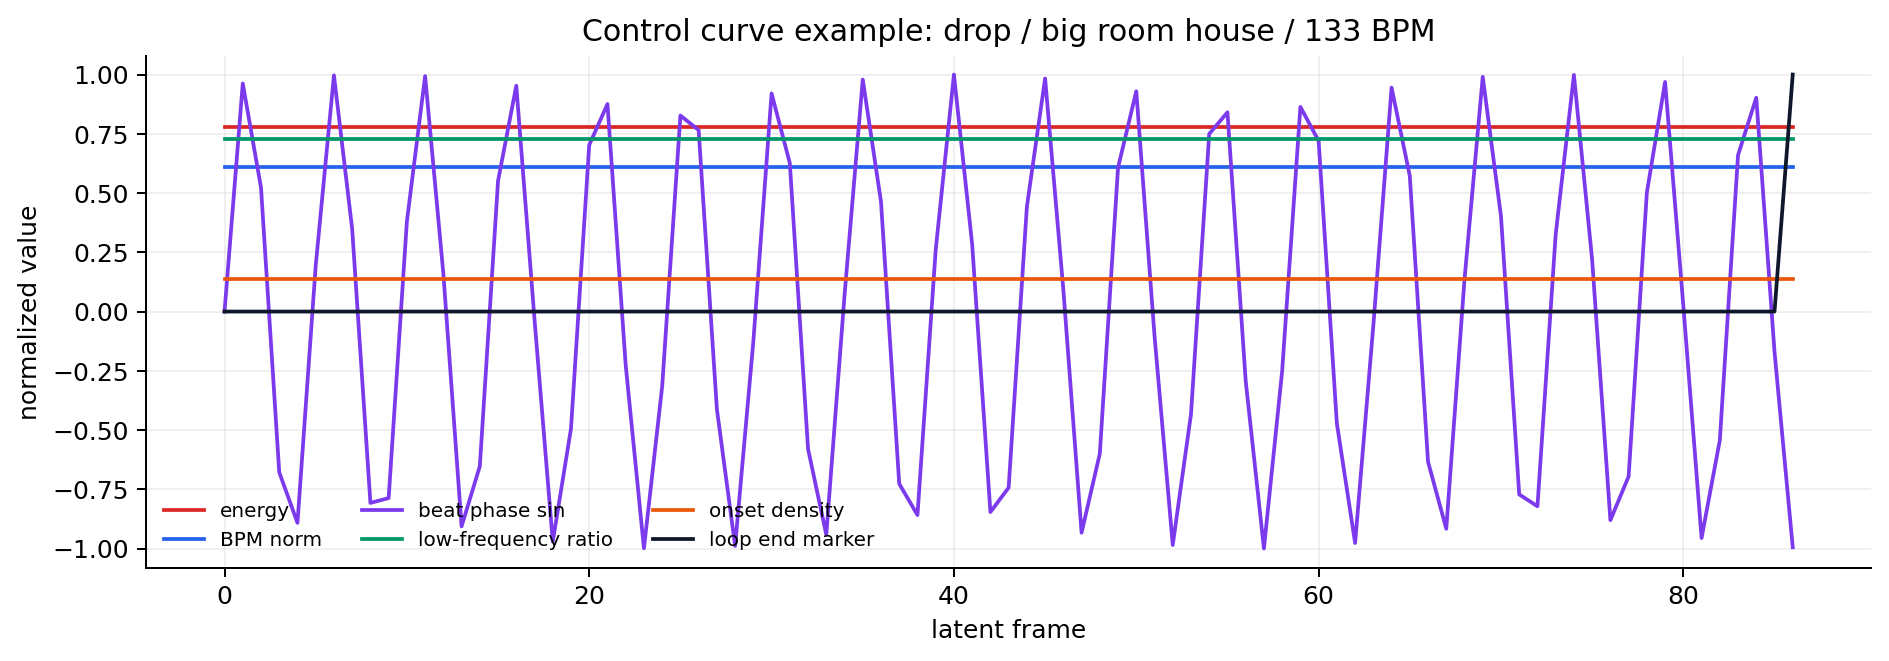
\includegraphics[width=0.92\linewidth]{../paper_assets/fig3_control_curve.png}
  \caption{latent 对齐 EDM 控制曲线示例}
  \label{fig:control_curve}
\end{figure}

\subsection{控制 token 投影器}

控制曲线 $C$ 不能直接输入文本编码序列，因此本文设计轻量 MLP control conditioner。首先对时间维进行自适应池化，将 $T$ 帧控制曲线压缩为 $K$ 个控制位置：
\begin{equation}
  \tilde{C} = \mathrm{Pool}(C) \in \mathbb{R}^{K \times F}.
\end{equation}
随后使用 LayerNorm、Linear、SiLU、Dropout 和 Linear 投影到文本 embedding 维度：
\begin{equation}
  Z_c = \mathrm{MLP}(\tilde{C}) + E_{type},\quad Z_c \in \mathbb{R}^{K \times d}.
\end{equation}
其中 $E_{type}$ 为可学习 token type embedding。当前实现中 $F=36$、$K=8$、$d=768$、hidden dimension 为 512。最终文本条件表示为：
\begin{equation}
  H' = [H_{text}; Z_c],
\end{equation}
其中 $H_{text}$ 为 UMT5 文本 embedding 输出。扩散 Transformer 以 $H'$ 作为条件序列，从而同时接收 prompt 语义与 EDM 结构控制。

\subsection{训练目标}

本文基于 ACE-Step 的扩散训练流程进行适配。在训练阶段，音频片段被编码为 latent $z_0$，并在扩散步 $t$ 上加入噪声得到 $z_t$。模型预测噪声或 velocity，训练目标可写为加权均方误差：
\begin{equation}
  \mathcal{L} =
  \mathbb{E}_{z_0,t,\epsilon}
  \left[
    w_i \left\|
      \epsilon - \epsilon_{\theta,\Delta\theta(m_i)}(z_t,t,H'_i)
    \right\|_2^2
  \right],
\end{equation}
其中 $w_i$ 为由质量分数和标签置信度计算的样本权重，$\Delta\theta(m_i)$ 表示由 router 激活的 LoRA 参数组合。基础模型主体参数保持冻结，仅训练 LoRA 参数和 control conditioner 参数，从而实现参数高效适配。

\section{系统实现}

\subsection{数据处理流水线}

项目实现了从原始音频到训练样本的完整流水线，如图 \ref{fig:pipeline} 所示。处理过程包括：原始音频收集、音频切片、EDM 元数据构建、音频特征分析、caption 生成、数据集划分、ACE-Step latent 缓存、text token 缓存、control curve 生成和 HuggingFace Dataset 转换。

\begin{figure}[H]
  \centering
  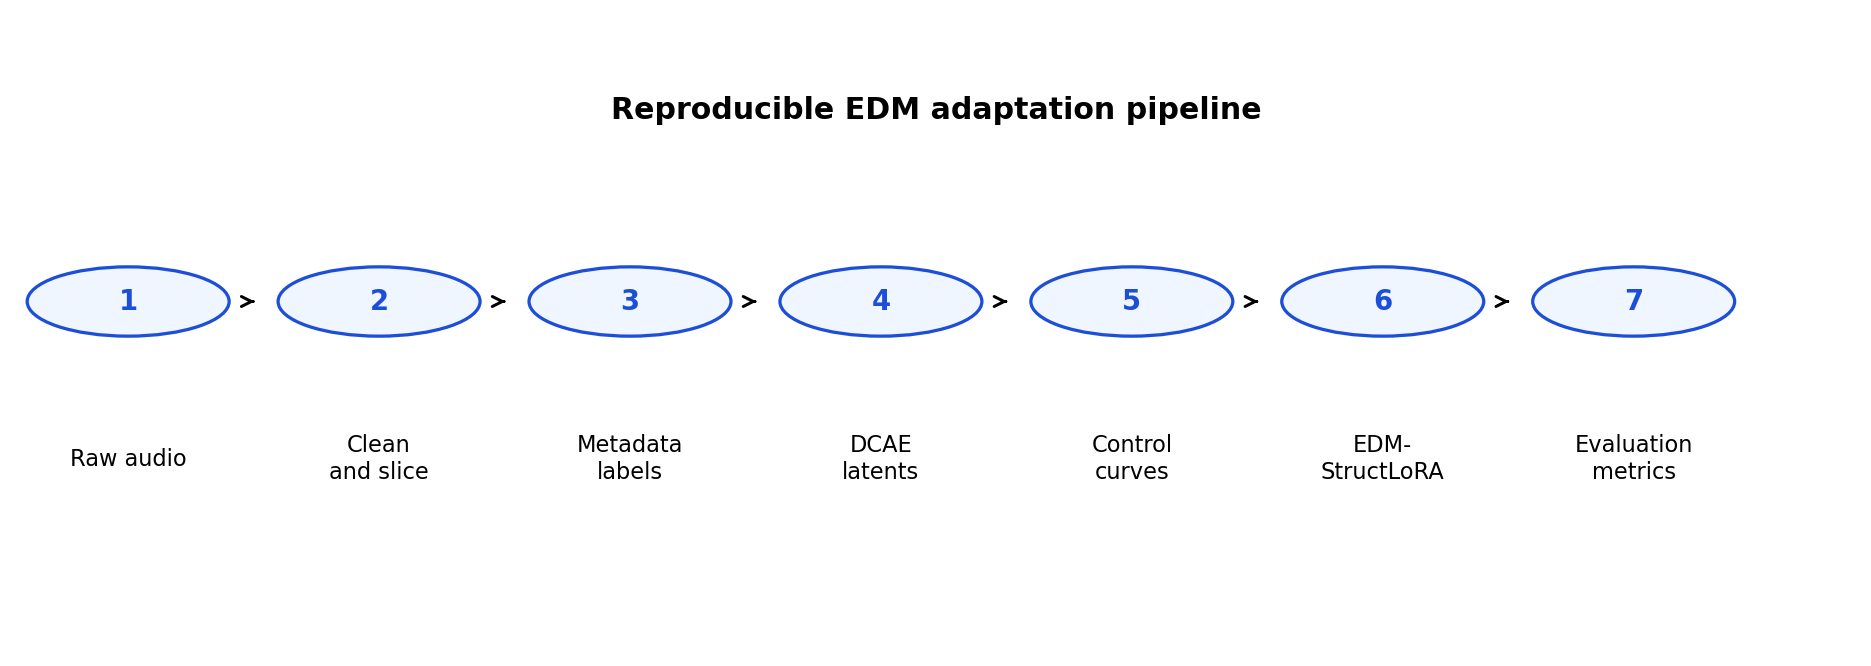
\includegraphics[width=0.92\linewidth]{../paper_assets/fig4_pipeline.png}
  \caption{EDM 数据处理与训练流水线}
  \label{fig:pipeline}
\end{figure}

每条样本包含音频路径、caption、section、energy、subgenre、BPM、质量分数、标签置信度、latent path、control path 和 text token path。训练时数据加载器优先读取缓存 latent，避免每个 step 重新执行音频编码，从而降低训练开销。

\subsection{数据集统计}

表 \ref{tab:dataset_summary} 给出了数据集规模。项目共包含 231 个原始音频源文件，其中 203 个完成有效处理，得到 6,016 条训练质量片段。所有片段长度为 8 秒，并按 train、validation 和 test 划分。

\begin{table}[H]
  \centering
  \caption{EDM 数据集规模统计}
  \label{tab:dataset_summary}
  \begin{tabular}{lc}
    \toprule
    项目 & 数值 \\
    \midrule
    原始音频源文件数 & 231 \\
    有效处理源文件数 & 203 \\
    训练质量片段数 & 6,016 \\
    训练集 / 验证集 / 测试集 & 4,833 / 557 / 626 \\
    单片段时长 & 8 s \\
    ACE-Step latents & 6,016 \\
    控制曲线 & 6,016 \\
    控制特征维度 & 36 \\
    \bottomrule
  \end{tabular}
\end{table}

图 \ref{fig:label_distribution} 展示了样本在子风格、段落和能量标签上的分布。可以看到，数据集中 drop 段落和 high/very\_high energy 样本占比较高，这符合 EDM 数据中高潮段落密集出现的特点，但也意味着后续实验需要关注类别不均衡带来的偏置。因此，本文在训练中加入 confidence-aware weighted sampling，以提高质量和置信度较高样本的贡献。

\begin{figure}[H]
  \centering
  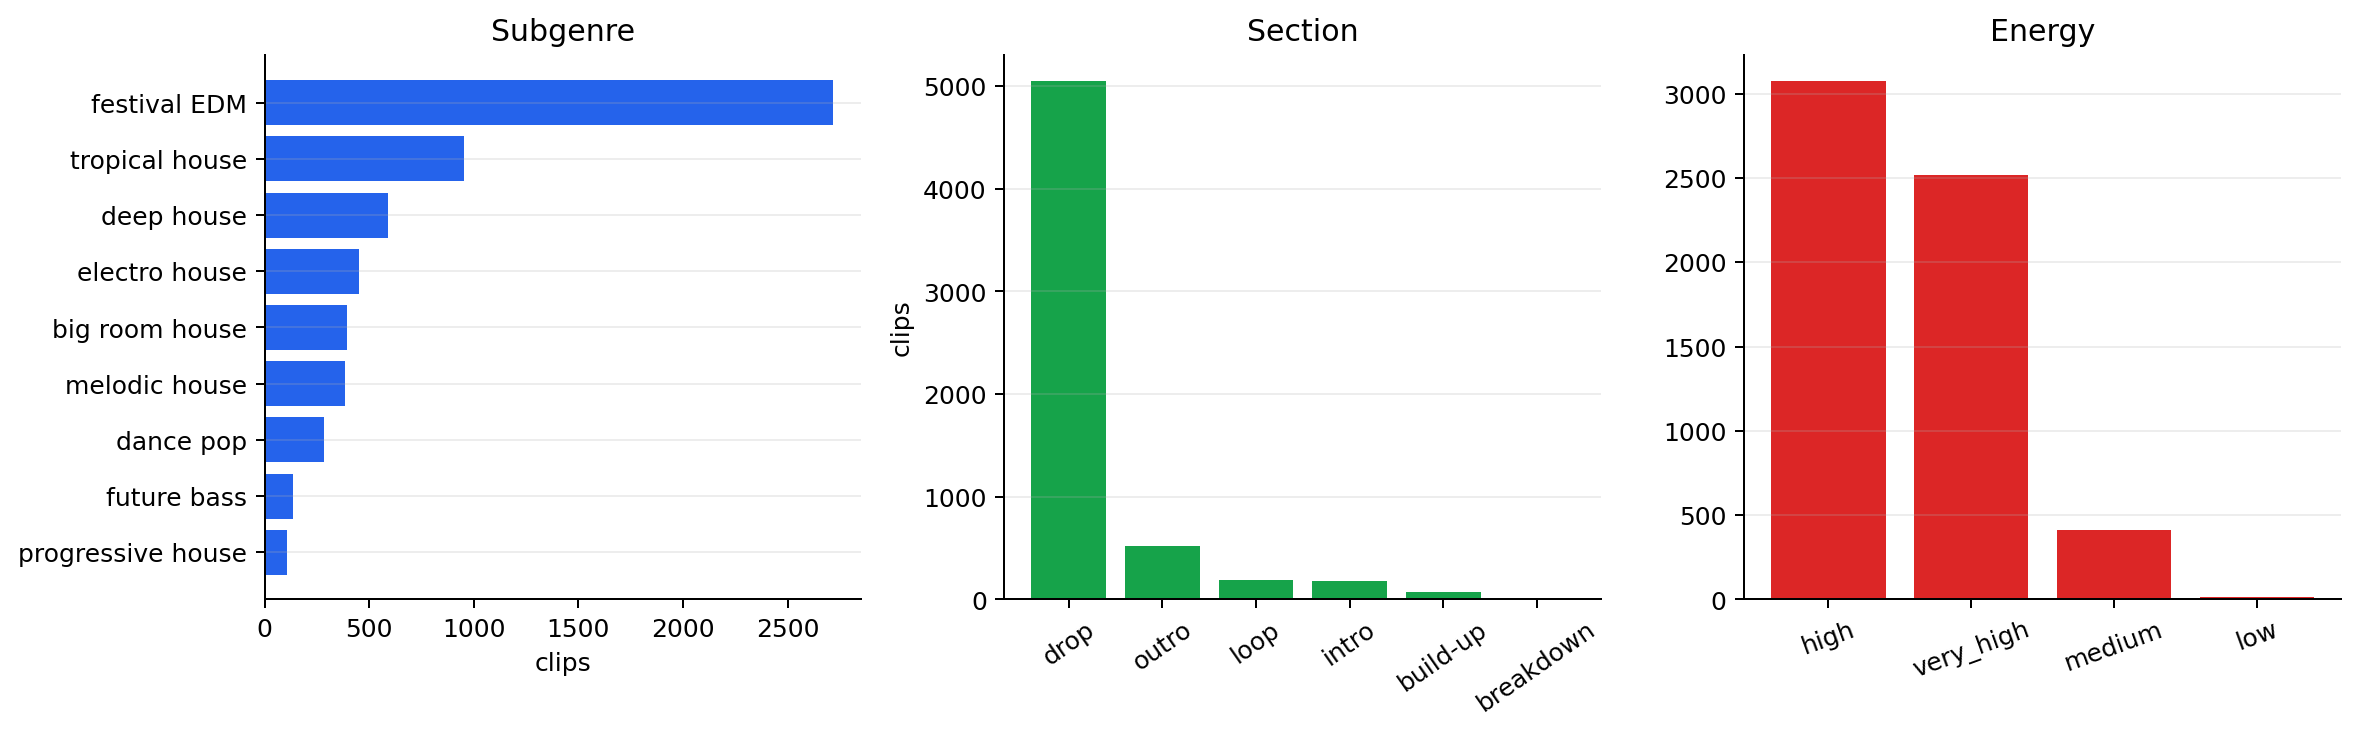
\includegraphics[width=0.92\linewidth]{../paper_assets/fig2_dataset_distribution.png}
  \caption{EDM 数据集标签分布}
  \label{fig:label_distribution}
\end{figure}

\subsection{模型配置}

表 \ref{tab:model_config} 给出了主要模型配置。共享 LoRA 使用 rank 32，专家 LoRA 使用 rank 8。两类 LoRA 均作用于 Transformer 注意力相关线性层，包括 linear\_q、linear\_k、linear\_v、to\_q、to\_k、to\_v 和 to\_out.0。训练采用 bf16-mixed 精度、梯度累积和 AdamW 优化器。

\begin{table}[H]
  \centering
  \caption{\modelname 关键配置}
  \label{tab:model_config}
  \begin{tabular}{ll}
    \toprule
    模块 & 配置 \\
    \midrule
    基础模型 & ACE-Step-v1-3.5B \\
    共享 LoRA & rank=32, alpha=16, rsLoRA \\
    专家 LoRA & rank=8, alpha=8, rsLoRA \\
    Adapter 数量 & 25 \\
    Router scale & section=0.90, energy=0.35, subgenre=0.45, BPM=0.20 \\
    Control conditioner & feature dim=36, token count=8, hidden dim=512 \\
    训练精度 & bf16-mixed \\
    推荐学习率 & $1\times10^{-4}$ \\
    梯度累积 & 8 \\
    采样策略 & confidence-aware weighted sampling \\
    \bottomrule
  \end{tabular}
\end{table}

\subsection{Adapter Bundle 与推理}

训练过程保存的不再是单个 LoRA 文件，而是包含 manifest、control conditioner 和多个 adapter 权重的 bundle。manifest 记录 adapter 名称、类型、路由配置、训练 step 和方法配置。推理时，系统加载基础 ACE-Step 模型和 LoRA bundle，根据用户输入的 section、energy、subgenre 和 BPM 计算路由权重，并注入控制 token 进行生成。

生成命令包含 prompt、lora bundle、duration、section、energy、subgenre、BPM、infer step 和 seed 等参数。生成完成后，系统同时保存 wav 音频和 JSON sidecar，用于记录 prompt、adapter 权重、控制参数和输出路径。这种设计有助于复现实验和分析不同控制条件下的生成行为。

\section{实验设计与原型验证}

\subsection{对照实验设计}

为验证各模块贡献，本文设计表 \ref{tab:ablation} 所示消融实验。A0 为未适配基础模型，A1 为普通 LoRA，A2 验证 metadata-rich caption 是否足以提供控制，A3 引入 section-aware LoRA，A4 加入 section 与 attribute router，A5 为完整 \modelname。

\begin{table}[H]
  \centering
  \caption{消融实验设计}
  \label{tab:ablation}
  \begin{tabular}{lll}
    \toprule
    编号 & 系统 & 实验目的 \\
    \midrule
    A0 & ACE-Step base & 未适配基线 \\
    A1 & Plain LoRA r=64 & 参数高效领域适配基线 \\
    A2 & Metadata-rich caption LoRA & 验证 caption 工程是否足够 \\
    A3 & Section-aware LoRA & 验证段落专家 adapter 的作用 \\
    A4 & Section + attribute routed LoRA & 验证动态路由机制 \\
    A5 & Full EDM-StructLoRA & 验证 router + control token + weighted sampling \\
    \bottomrule
  \end{tabular}
\end{table}

\subsection{评价指标}

EDM 生成评价不能只依赖主观听感。本文建议从结构可控性、节奏一致性、音频质量和人工评价四类指标进行综合分析，如表 \ref{tab:metrics} 所示。

\begin{table}[H]
  \centering
  \caption{建议评价指标}
  \label{tab:metrics}
  \begin{tabular}{lp{9.2cm}}
    \toprule
    指标 & 含义 \\
    \midrule
    BPM Error & 目标 BPM 与生成音频估计 BPM 的绝对误差 \\
    Onset Density Error & 目标鼓点密度与生成鼓点密度之间的差异 \\
    Low-frequency Ratio & 低频能量占比，用于衡量 drop 或 bass-heavy 片段表现 \\
    Loop Similarity & loop 首尾频谱或 embedding 相似度，用于衡量循环可用性 \\
    Section Controllability & 目标 section 与分类器预测 section 的一致性 \\
    Text-audio Similarity & 文本提示与生成音频 embedding 的相似度 \\
    FAD / Embedding Distance & 生成分布与参考 EDM 数据分布之间的距离 \\
    Human Blind Test & 风格匹配、drop 冲击、loop 可用性和总体音质评分 \\
    \bottomrule
  \end{tabular}
\end{table}

\subsection{原型验证结果}

当前原型已完成方法实现和系统级验证，具体包括：

\begin{enumerate}[leftmargin=2em,itemsep=0.2em]
  \item 完成 6,016 条 EDM 片段的 metadata、caption、latent、control curve 和 text token 构建，control assets 覆盖率为 6,016/6,016。
  \item 完成 train/validation/test 数据划分，并将训练集转换为 HuggingFace Dataset 格式，训练样本数为 4,833。
  \item 实现动态 LoRA router，可根据 batch metadata 输出 shared、section、energy 和 subgenre adapter 权重。
  \item 实现 control conditioner，将 36 维帧级控制序列压缩为 8 个文本条件 token，并拼接至 UMT5 embedding。
  \item 完成 step=1000 的 EDM control LoRA bundle 保存，bundle 内包含 25 个 adapter 权重、manifest 和 control conditioner。
  \item 实现可控推理脚本，可根据用户输入的 prompt、section、energy、subgenre 和 BPM 动态加载 adapter mixture 并生成音频。
\end{enumerate}

需要说明的是，本文当前阶段重点是方法设计、系统实现和可复现实验框架构建。若用于正式投稿，还需要补充完整主观听测、自动指标和多基线消融结果。本文已经在实验设计层面给出了可直接执行的比较方案和指标体系，后续可在同一代码框架下扩展最终量化结果。

\section{讨论}

\subsection{方法优势}

\modelname 的主要优势在于将 EDM 音乐制作知识显式融入模型适配过程。普通 LoRA 学习的是平均域偏移，容易把不同段落、能量和子风格混合为单一风格特征。本文通过专家 adapter 和 router 将结构差异映射到不同低秩参数子空间，使模型能够在生成时根据条件进行参数级切换。另一方面，control curve 将 BPM、beat phase、onset density 和 loop boundary 等时间信号显式注入条件序列，弥补了 prompt 对连续控制表达不足的问题。

\subsection{局限性}

当前原型仍存在三方面局限。第一，数据分布存在不均衡，drop 和 high energy 样本占比较高，breakdown 等少数段落样本不足。第二，本文采用启发式 router scale，虽然便于解释和调试，但尚未学习到最优路由函数。第三，当前控制 token 使用平均池化压缩控制曲线，可能损失部分细粒度时间变化信息。未来可探索可学习 temporal attention、router 正则化和类别均衡采样，以进一步提高控制精度。

\subsection{潜在应用}

该系统可用于短视频背景音乐、游戏循环音乐、DJ loop 草稿、电子音乐制作灵感辅助、广告配乐和风格化音频素材生成。与普通文本生成音乐相比，\modelname 更适合需要明确 BPM、段落和能量控制的制作型场景。

\section{结论}

本文提出 \modelname，一种面向 EDM 文本生成音乐的结构与属性感知参数高效适配方法。该方法基于 ACE-Step 音乐生成基础模型，将 LoRA 从单一 adapter 扩展为共享 EDM adapter、section experts、energy experts 和 subgenre experts，并通过元数据路由器动态激活 adapter mixture。同时，本文构建 latent 对齐控制曲线，将 EDM 的段落、BPM、节拍相位、低频能量、onset 密度、loop 边界和置信度编码为显式控制信号，再投影为控制 token 注入文本条件序列。项目实现了包含 6,016 条 EDM 片段的数据处理、训练、保存和推理闭环，为可控 EDM 生成提供了可复现的研究原型。未来工作将围绕完整量化评测、人工盲听实验、可学习 router 和更细粒度时间控制展开。

\begin{thebibliography}{99}

\bibitem{lora}
E. J. Hu, Y. Shen, P. Wallis, Z. Allen-Zhu, Y. Li, S. Wang, L. Wang, and W. Chen,
``LoRA: Low-Rank Adaptation of Large Language Models,''
arXiv:2106.09685, 2021.

\bibitem{musicgen}
J. Copet, F. Kreuk, I. Gat, T. Remez, D. Kant, G. Synnaeve, Y. Adi, and A. Défossez,
``Simple and Controllable Music Generation,''
arXiv:2306.05284, 2023.

\bibitem{musiclm}
A. Agostinelli, T. Denk, Z. Borsos, J. Engel, M. Verzetti, A. Caillon, Q. Huang, A. Jansen, A. Roberts, M. Tagliasacchi, M. Sharifi, N. Zeghidour, and C. Frank,
``MusicLM: Generating Music From Text,''
arXiv:2301.11325, 2023.

\bibitem{audioldm}
H. Liu, Z. Chen, Y. Yuan, X. Mei, X. Liu, D. Mandic, W. Wang, and M. D. Plumbley,
``AudioLDM: Text-to-Audio Generation with Latent Diffusion Models,''
arXiv:2301.12503, 2023.

\bibitem{controlnet}
L. Zhang, A. Rao, and M. Agrawala,
``Adding Conditional Control to Text-to-Image Diffusion Models,''
Proceedings of the IEEE/CVF International Conference on Computer Vision, 2023.

\bibitem{musicongen}
Y.-H. Lan, W.-Y. Hsiao, H.-C. Cheng, and Y.-H. Yang,
``MusiConGen: Rhythm and Chord Control for Transformer-Based Text-to-Music Generation,''
arXiv:2407.15060, 2024.

\bibitem{ddpm}
J. Ho, A. Jain, and P. Abbeel,
``Denoising Diffusion Probabilistic Models,''
Advances in Neural Information Processing Systems, 2020.

\bibitem{acestep}
ACE-Step Team,
``ACE-Step: A Step Towards Music Generation Foundation Model,''
arXiv:2506.00045, 2025.

\end{thebibliography}

\end{document}
